\documentclass[10pt,a4paper]{report}
\usepackage[left=3.00cm, right=1.00cm, top=2.00cm, bottom=2.00cm, nohead, footskip=7mm]{geometry}
\usepackage[14pt]{extsizes}

\usepackage[utf8]{inputenc}
\usepackage[T1]{fontenc}
\usepackage{amsmath}
\usepackage{amsfonts}
\usepackage{amssymb}
\usepackage{pdfpages}

\usepackage[russian]{babel}

% Ссылки внутри текста
\usepackage{hyperref}

% Отступ абзаца
\usepackage{indentfirst}
\setlength{\parindent}{1.5cm} 

% Межстрочный интервал
\usepackage{setspace}
\onehalfspacing % интервал 1.5

% Вставка изображений
\usepackage{graphicx}
\graphicspath{{../schemes/}}

% Настройка оглавлений
\usepackage{titlesec}
\newcommand{\hsp}{\hspace{20pt}}
\titleformat{\chapter}[hang]{\large\bfseries}{\thechapter{. }}{0pt}{\large\bfseries}
\titlelabel{hlabel-formati}
\titlespacing{\chapter}{42pt}{-80pt}{12pt}
\titleformat{\section}[hang]{\large\bfseries}{\thesection{. }}{0pt}{\large\bfseries}
\titlespacing{\section}{42pt}{12pt}{5pt plus 5pt}

% Настройка списков
\usepackage{enumitem}
\setlist{nolistsep, itemsep=0.3cm,parsep=0pt,leftmargin=1.9cm}

% Настройка листингов
\usepackage{listings}
\lstset{
	language = c++,
	extendedchars=\true,
	keepspaces=true,
	basicstyle=\small\sffamily,
	showstringspaces=\false,
	numbers=left,
	stepnumber=1,
	numbersep=5pt,
	frame=single,
	tabsize=2,
	captionpos=t,
	breaklines=true,
	breakatwhitespace=false,
	escapeinside={\#*}{*)}
}



\begin{document}
	\renewcommand\bibname{Список литературы}
	
	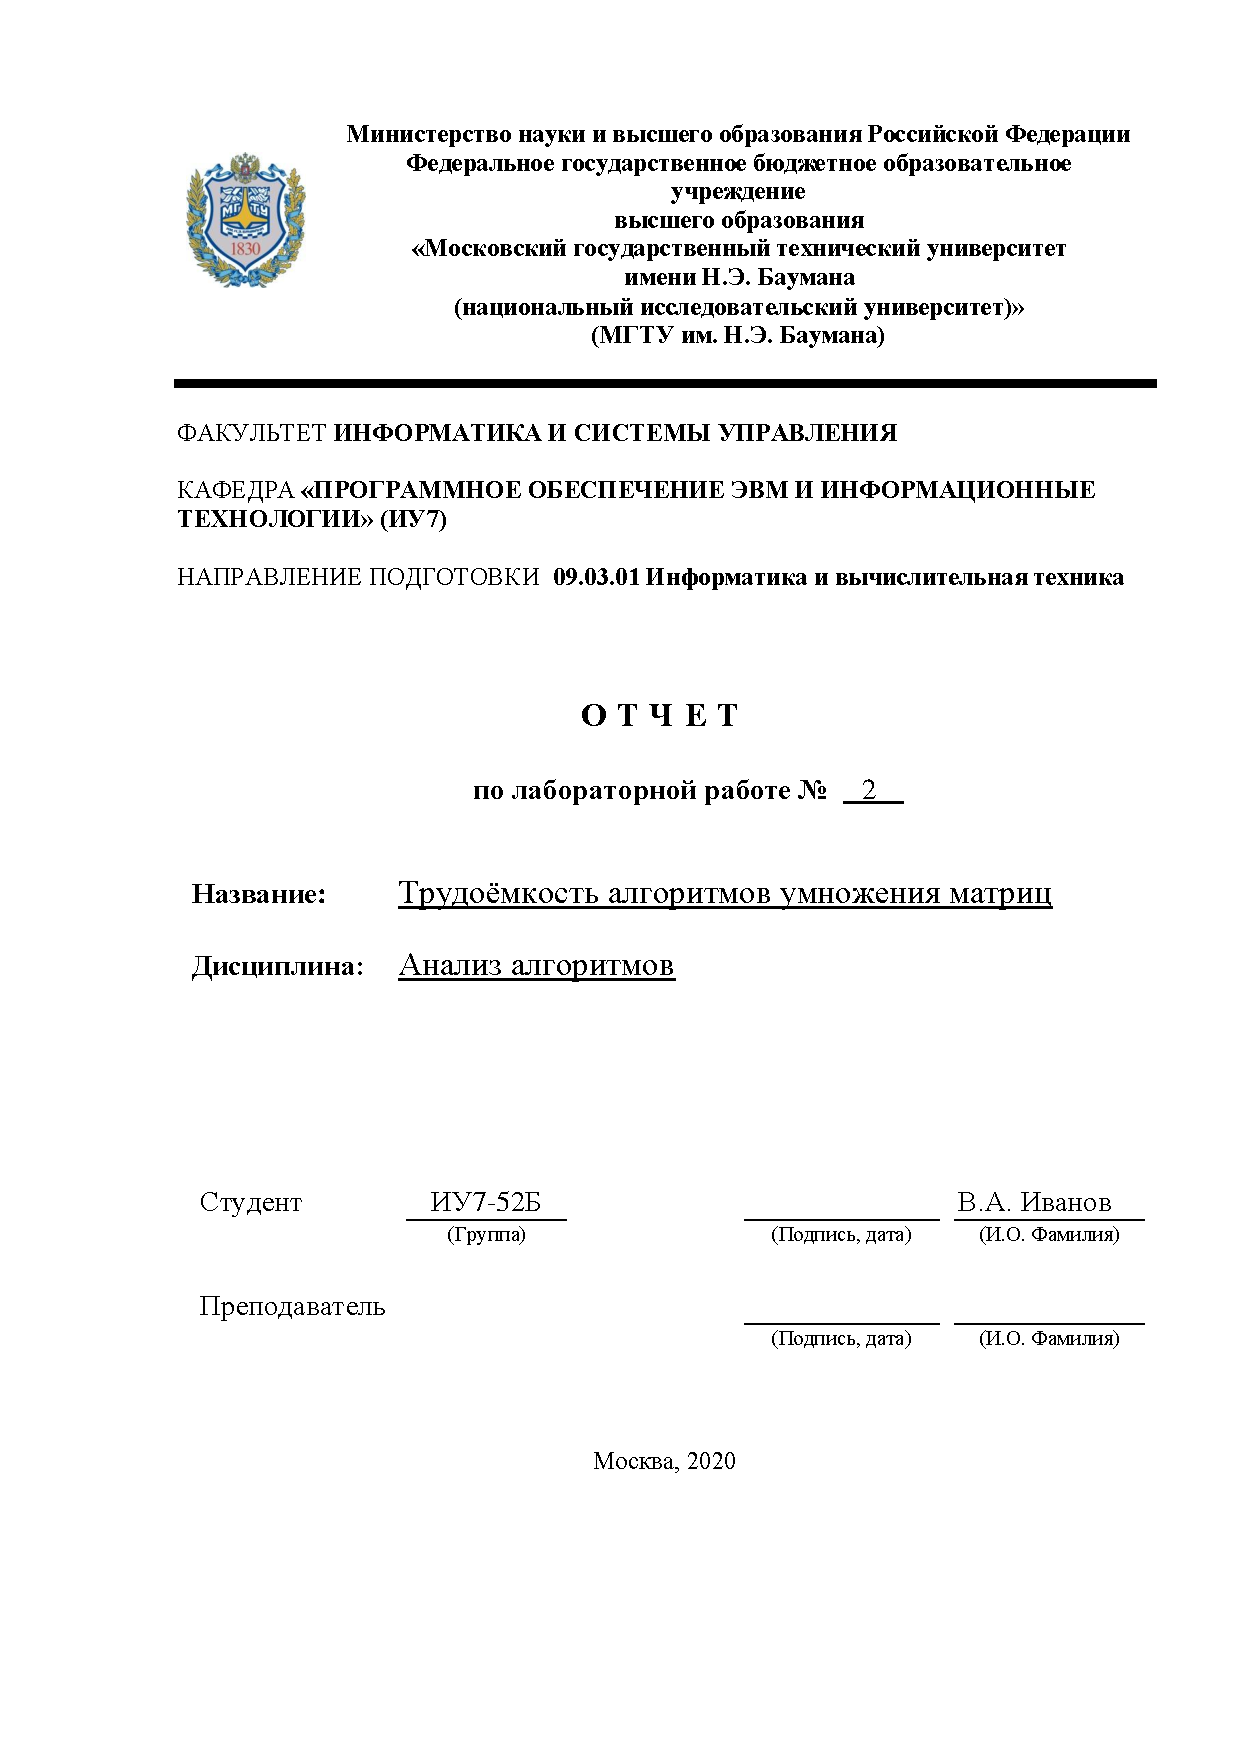
\includepdf[pages=1]{title.pdf}
	
	\tableofcontents
	\newpage

	\chapter*{Введение}
	\addcontentsline{toc}{chapter}{Введение}
	В данной лабораторной реализуются и оцениваются различные алгоритмы поиска ключей в словаре банковских карт.

Словари используются для связывания двух понятий, одно из которых называется ключом, а другое значением. Сам словарь хранит множество таких пар и предоставляет определённые функции для работы с хранимыми значениями. Одной из самых часто используемых операций в таком случае является операция получения значения по заданному ключу. В случае, когда словарь имеет большое количество записей, например более одного миллиона, задача уменьшения времени поиска ключей становится особенно актуальной. Поэтому существует множество алгоритмов, осуществляющих данную задачу.

В данной лабораторной работе в качестве примера подобных алгоритмов будут рассмотрены:
\begin{itemize}
	\item поиск полным перебором;
	\item поиск половинным делением;
	\item поиск полным перебором с использованием сегментации;
\end{itemize}

	\newpage

	\chapter{Аналитическая часть}
	Целью лабораторной работы является оценка трудоёмкости алгоритма умножения матриц и получение
практического навыка оптимизации алгоритмов.

Выделены следующие задачи лабораторной работы:

\begin{itemize}
\item математическое описание операции умножения матриц;
\item описание и реализация алгоритмов умножения матриц;
\item описание применённых к алгоритму Винограда способов оптимизации;
\item проведение замеров процессорного времени работы алгоритмов при различных размерах матриц 
(серия экспериментов для чётного размера и для нечётного);
\item оценка трудоёмкости алгоритом;
\item проведение сравнительного анализа алгоритмов на основании экспериментов.
\end{itemize}

Умножение матриц - операция над матрицами $ А[MxN] $ и $ B[NxQ] $. Результатом операции является матрица C размерами $ M*Q $, в которой элемент $c_{i,j}$ задаётся формулой
\begin{equation} 
	c_{i,j} = \sum_{k=1}^{N}(a_{i,k} \cdot b_{k,j})
\end{equation}


	\newpage
	
	\chapter{Конструкторская часть}
	Рассмотрим вышеупомянутые алгоритмы сортировки. Для удобства изложения сути алгоритмов, будем рассматривать сортировку по неубыванию. Алгоритмы сортировки других порядков могут быть получены заменой условия сравнения.

\section{Сортировка пузырьком}
Алгоритм сортировки пузырьком основывается на следующем действии. Массив проссматривается от 0 до N-2 элемента, и в случае, если текущий элемент массива больше следующего, они меняются местами. Таким образом, после первого прохода в конце массива окажется максимальный элемент, после второго - два максимальных, и так далее до полного упорядочивания массива.

Схема алгоритма приведена на рисунке 2.1.
\begin{figure}[h]
	\begin{center}
		{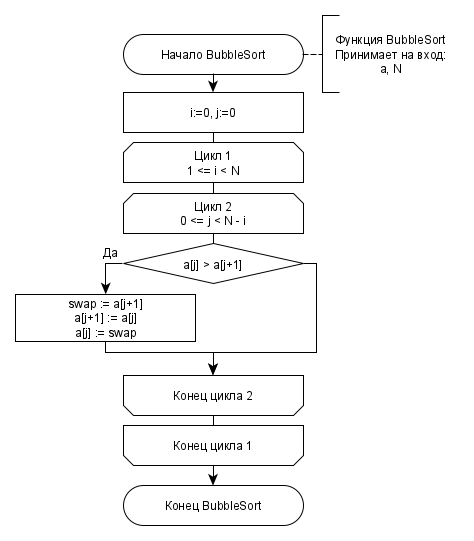
\includegraphics[height=20cm, width = 17cm]{Bubble}}
		\caption{Сортировка пузырьком}
	\end{center}
\end{figure}


\section{Поразрядная сортировка}
Цель алгоритма заключается в реализации трудоёмкости, линейно зависящей от размера массива. Упорядоченнсть достигается последовательной сортировкой по значению разрядов (в порядке от меньшего разряда к большему). Алгоритм применим к массиву, состоящему из целых положительных чисел или иных значений, которые м.б. спроецированы на множетво положительных чисел \cite{Korman}. 

Будем считать, что максимальное число в массиве состоит из K разрядов. В случае, если массив содержит целыйе отрицательные числа, то перед сортировкой все числа должны быть увеличены на модуль минимального числа, а после сортировки уменьшены.

Схема алгоритма приведена на рисунках 2.2. и 2.3.
\begin{figure}[h]
	\begin{center}
		{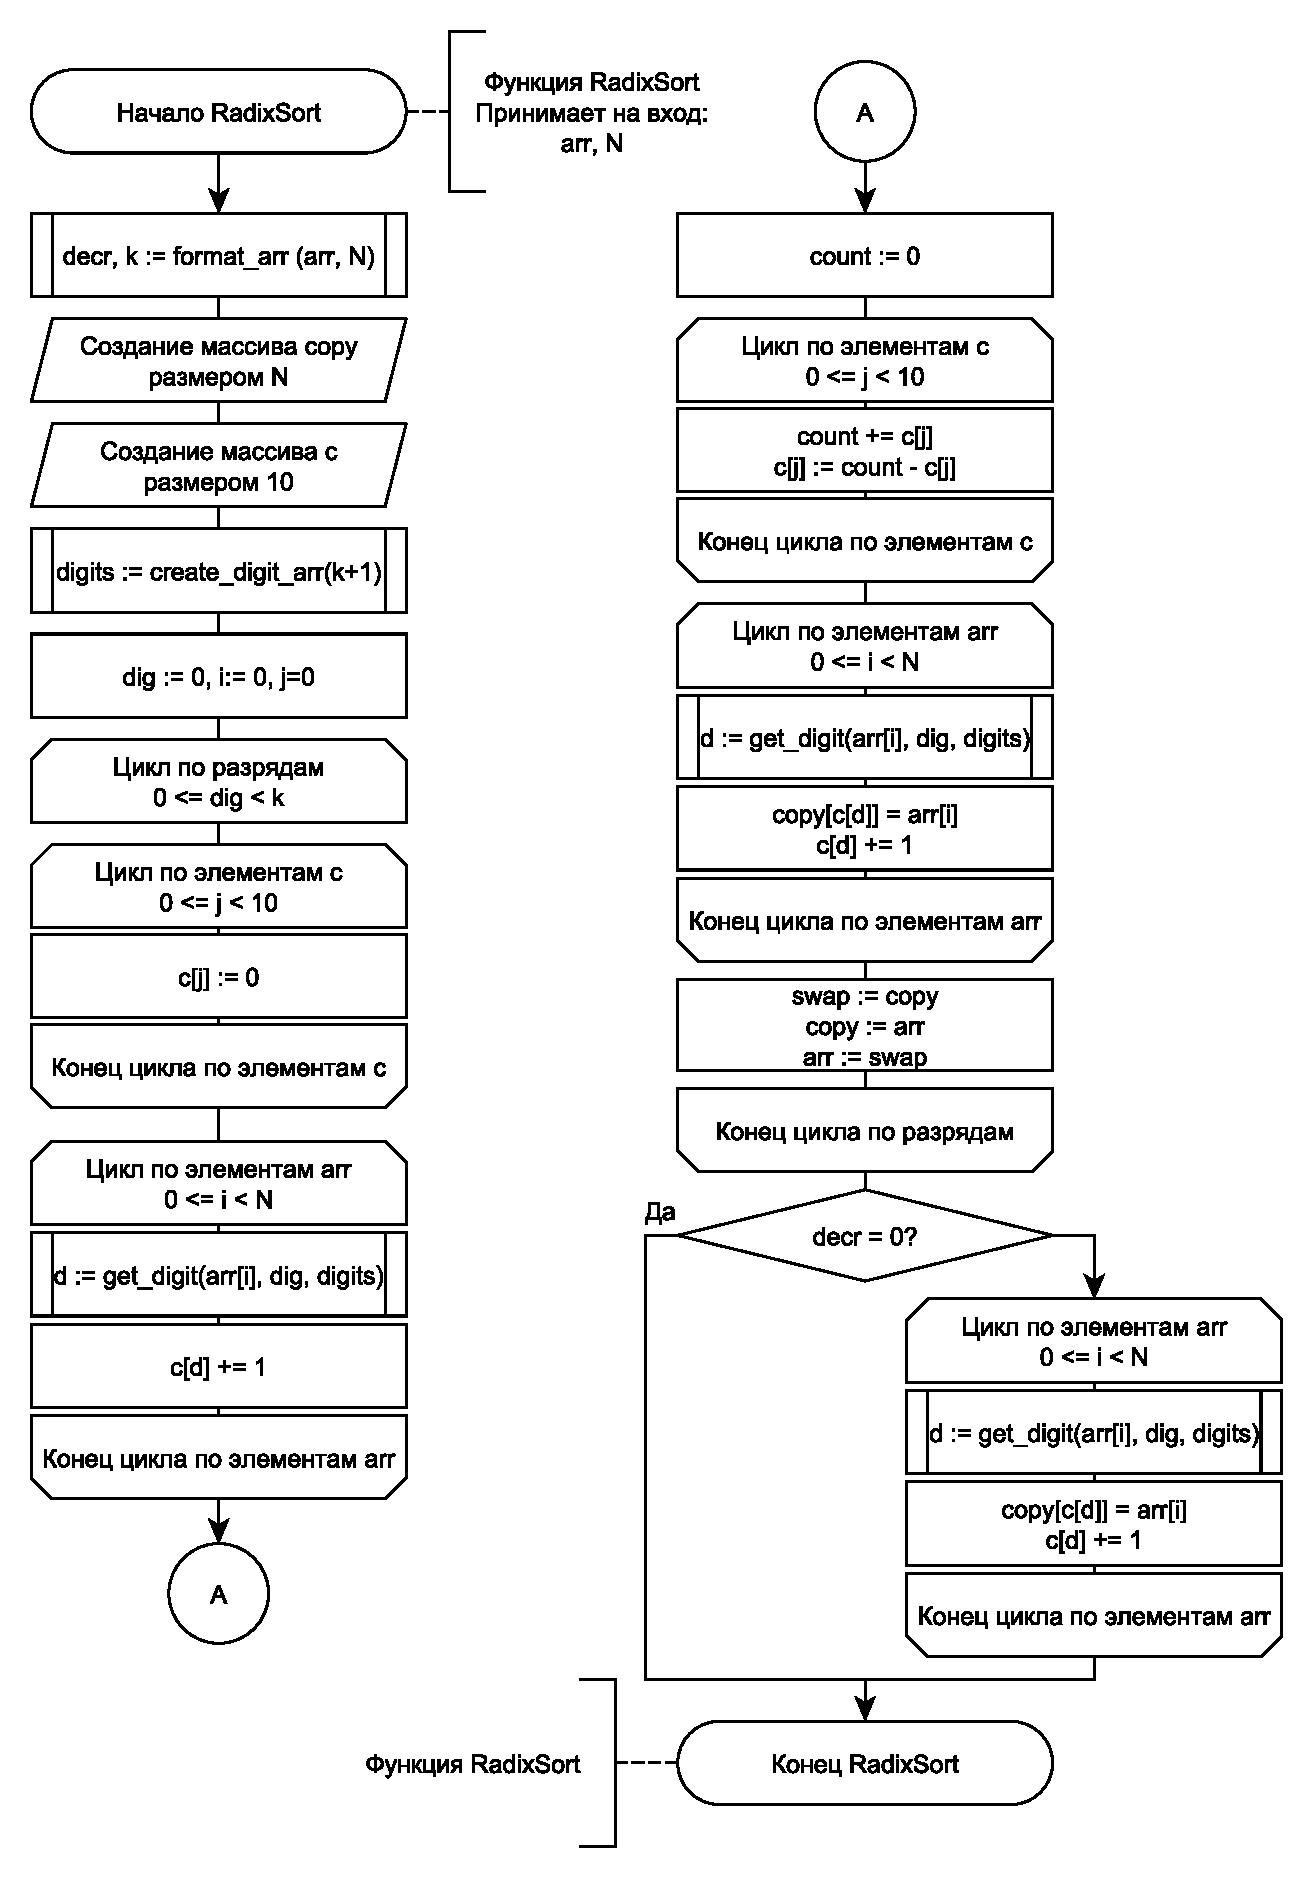
\includegraphics[height=20cm]{Radix1}}
		\caption{Поразрядная сортировка (часть 1)}
	\end{center}
\end{figure}

\begin{figure}[h]
	\begin{center}
		{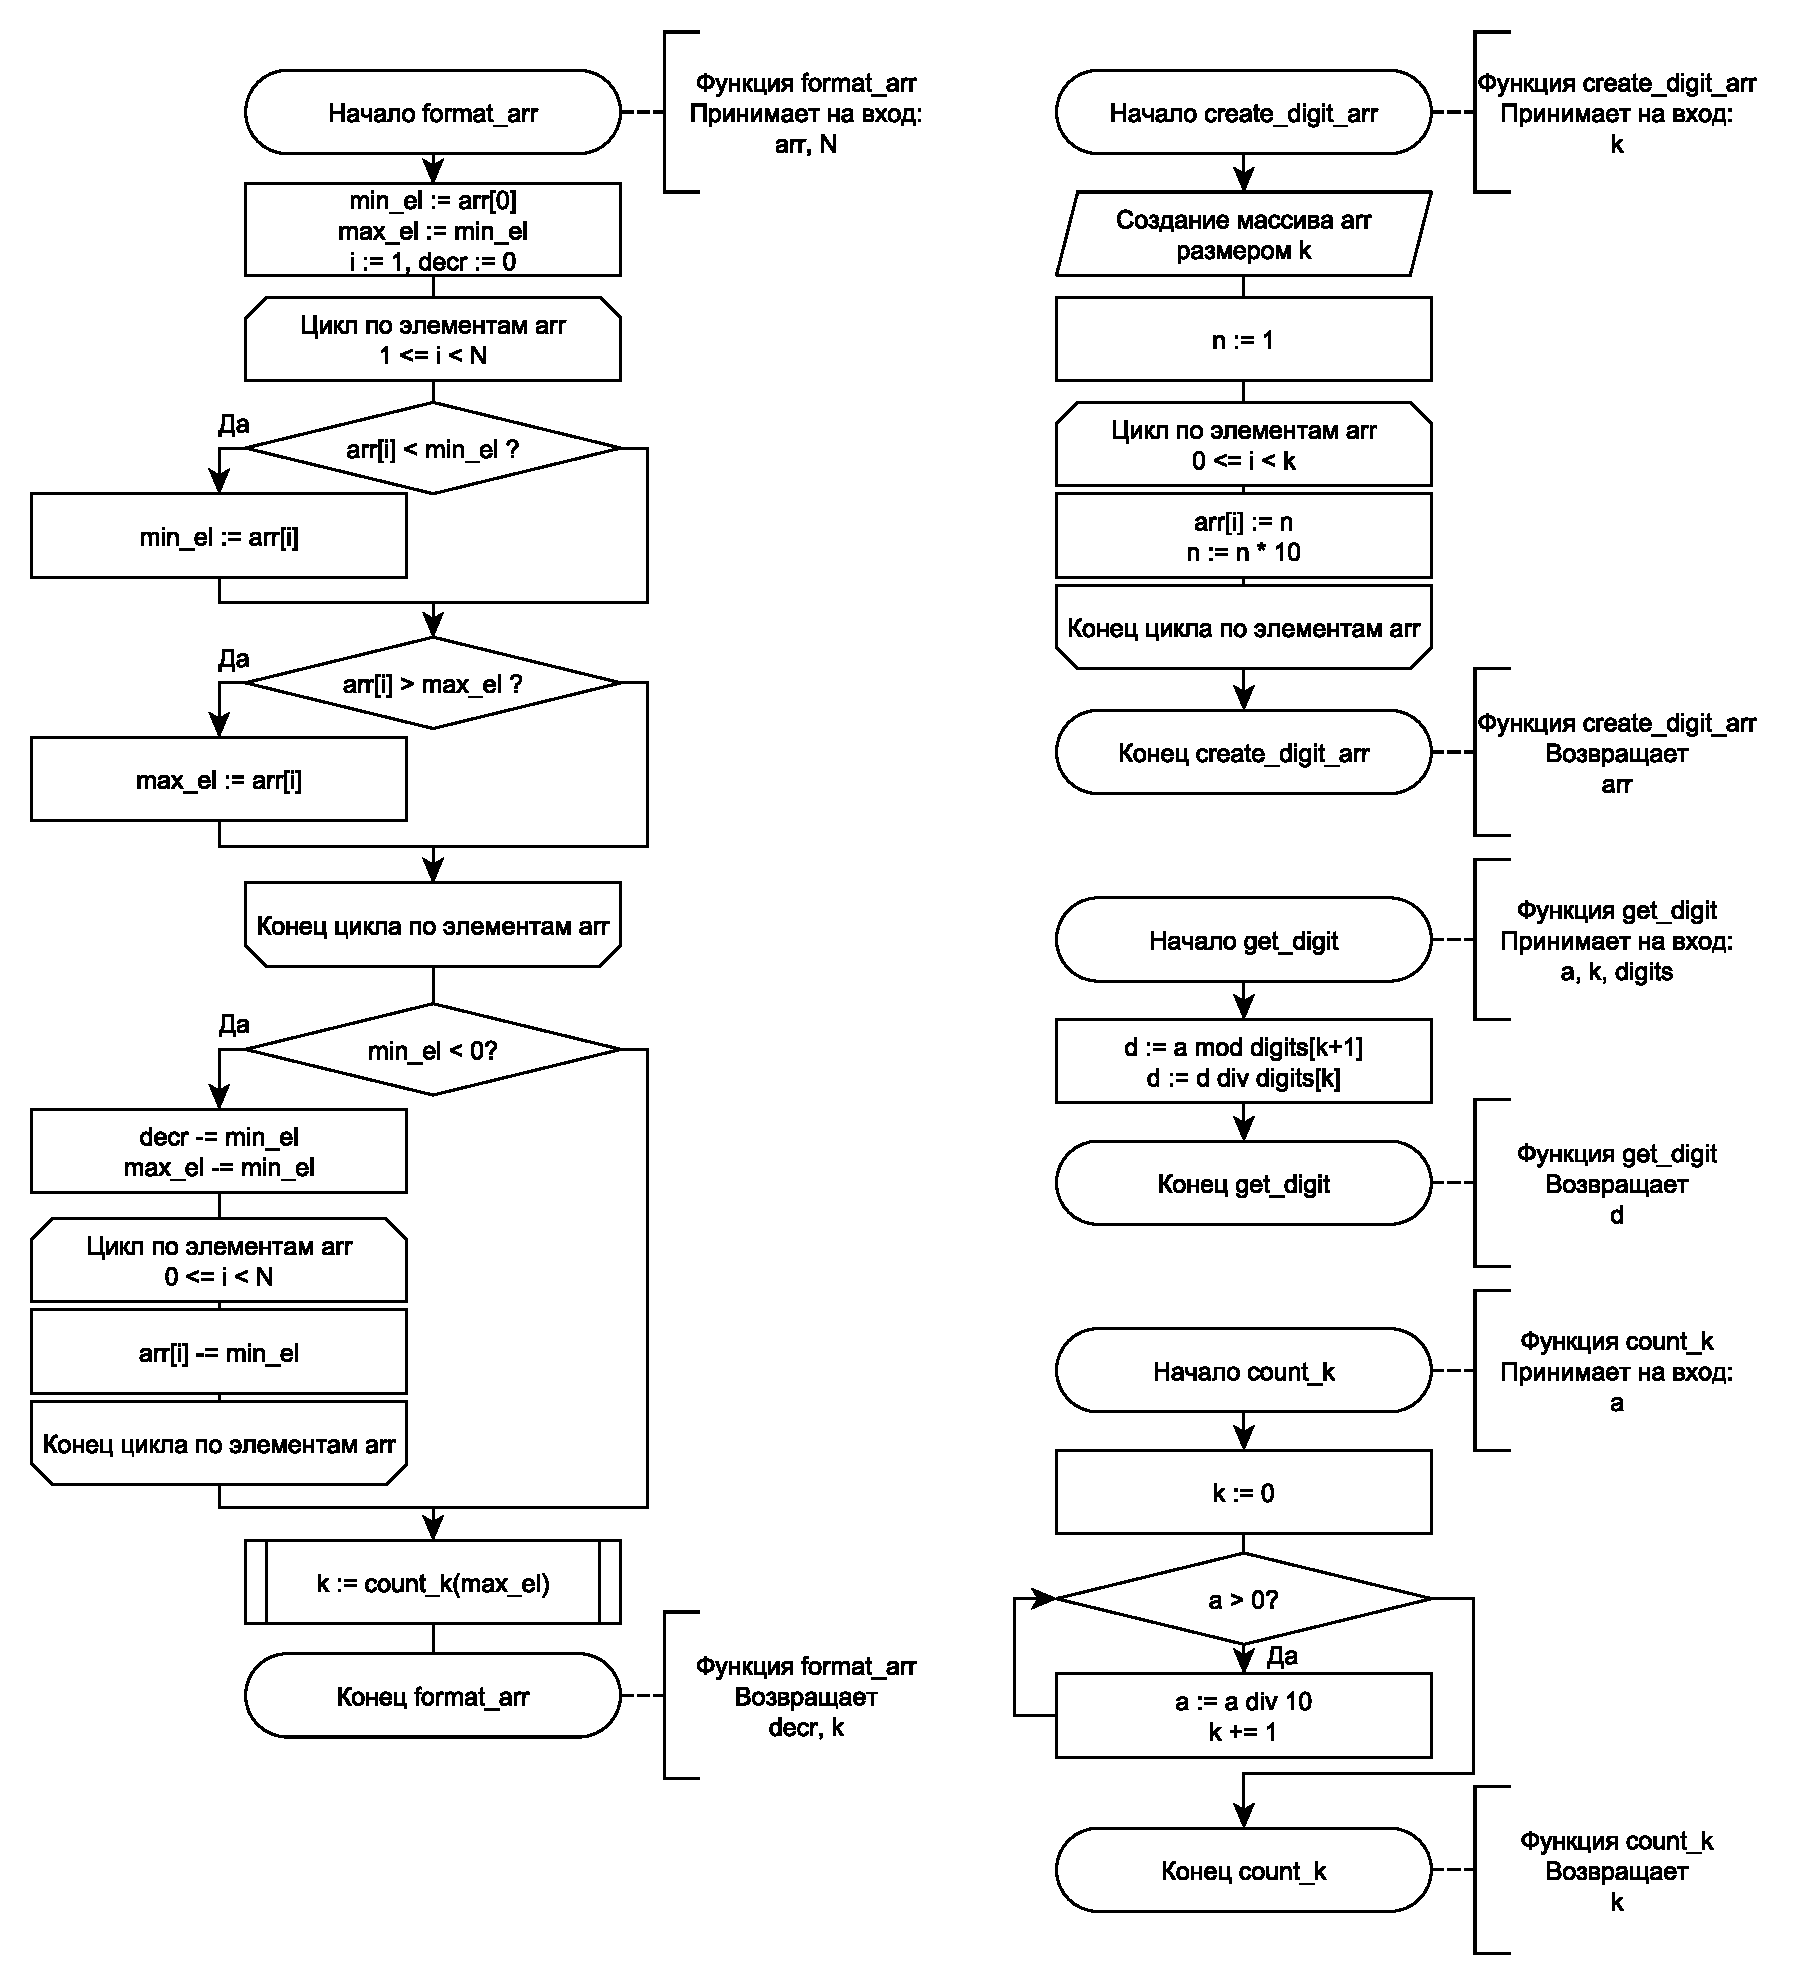
\includegraphics[width = 17cm]{Radix2}}
		\caption{Поразрядная сортировка (часть 2)}
	\end{center}
\end{figure}


\section{Сортировка слиянием}
Идея алгоритма заключается в том, что достаточно эффективно производится операция слияния (т.е. создания из двух массивов одного) при условии, что оба сливаемых массива уже упорядочены. Алгоритм разбивает массив на два подмассива, после чего применяет к ним ту же операцию, до тех пор, пока длина массива не станет меньше 3. После завершения сортировки подмассивов производится построение упорядоченного массива их слиянием.

Схема алгоритма приведена на рисунке 2.4.
\begin{figure}[h]
	\begin{center}
		{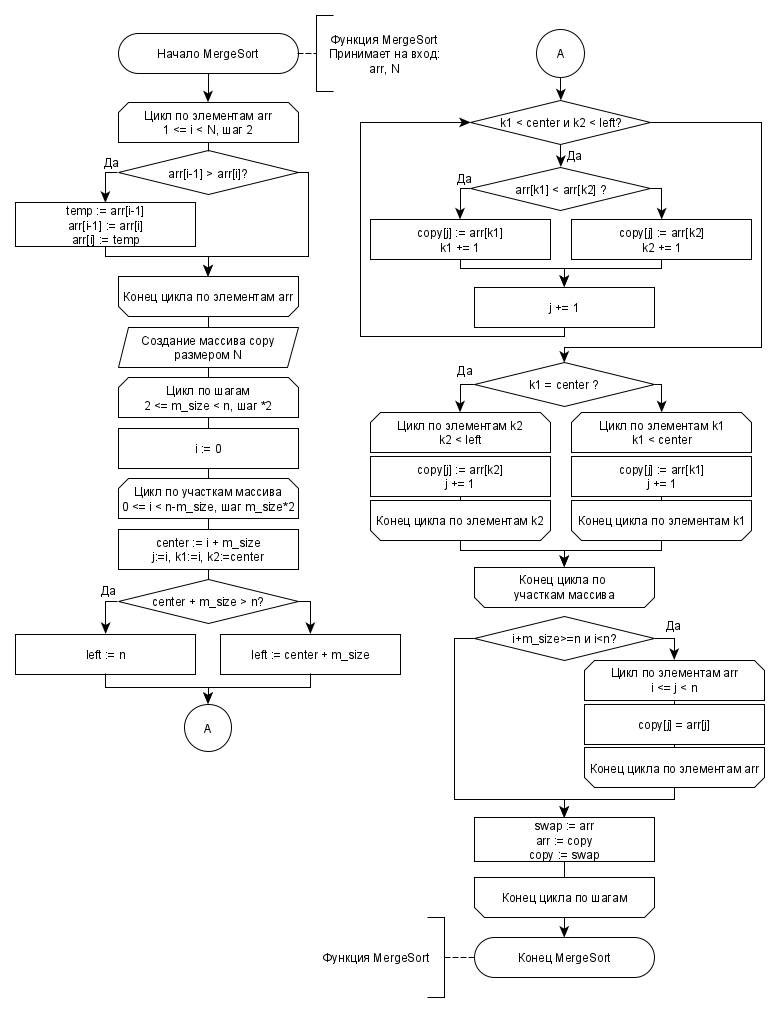
\includegraphics[height=20cm]{Merge}}
		\caption{Сортировка слиянием}
	\end{center}
\end{figure}


\section{Требования к программному обеспечению}
Для полноценной проверки и оценки алгоритмов необходимо выполнить следующее.
\begin{enumerate}
	\item Обеспечить возможность консольного ввода массива и выбора алгоритма сортировки. Программа должна вывести отсортированный массив.
	\item Реализовать функцию замера процессорного времени, затраченного функцией. Для этого также создать возможность ввода размера массива, на котором будет выполнен замер.
\end{enumerate}


\section{Заготовки тестов}
При проверке алгоритмов необходимо будет использовать следующие классы тестов:
\begin{itemize}
	\item массив размером 1;
	\item массив одинаковых элементов;
	\item упорядоченный и обратно упорядоченный массив.
\end{itemize}

\section*{Вывод}
Результатом конструкторской части стало схематическое описание алгоритмов сортировок, задание требований к программному обеспечению и к системе тестов.


	\newpage

	\chapter{Технологическая  часть}
	\section{Выбор языка программирования}
В качестве языка программирования был выбран C++\cite{C++_Doc}, так как имеется опыт работы с ним, и с библиотеками, позволяющими провести исследование и тестирование программы. Разработка проводилась в среде Visual Studio 2019\cite{VisualStudio}.

\section{Листинги кода}
Реализация алгоритмов поиска представлена на листингах 3.1-3.3. На листинге 3.4 представлена реализация разбиения словаря по сегментам

\begin{lstlisting}[caption = {Поиск полным перебором}]
rec_t full_search(const rec_arr& arr, size_t key)
{
	for (int i = 0; i < arr.size(); i++)
		if (arr[i].key == key)
			return arr[i];
	return null_rec();
}
\end{lstlisting}

\begin{lstlisting}[caption = {Поиск половинным разбиением}]
rec_t binary_search(const rec_arr& arr, size_t key)
{
	int left = 0;
	int right = arr.size() - 1;
	while (left <= right)
	{
		int mid = (left + right) / 2;
		if (key == arr[mid].key)
			return arr[mid];
		if (key < arr[mid].key)
			right = mid - 1;  
		else                  
			left = mid + 1;   
	}
	return null_rec();
}
\end{lstlisting}

\begin{lstlisting}[caption = {Поиск с сегментами}]
rec_t segment_search(const seg_arr& segments, size_t key)
{
	int seg_n = -1;
	for (int i=0; i<segments.size(); i++)
	if (segments[i].key == key % 10)
	{
		seg_n = i;
			break;
	}
	
	if (seg_n == -1)
		return null_rec();
	
	const rec_arr& arr = segments[seg_n].records;
	return full_search(arr, key);
}
\end{lstlisting}

\begin{lstlisting}[caption = {Разбиение словаря по сегментам}]
seg_arr split_arr(rec_arr& arr)
{
	seg_arr segments;
	for (int i = 0; i < 10; i++)
	{
		rec_seg temp_seg;
		temp_seg.key = i;
		
		segments.push_back(temp_seg);
	}
	
	for (int i = 0; i < arr.size(); i++)
		segments[arr[i].key % 10].records.push_back(arr[i]);
	return segments;
}
\end{lstlisting}


\section{Результаты тестирования}
Для тестирования написанных функций был создан отдельный файл с ранее описанными классами тестов. Тестирование функций проводилось за счёт сравнения результов функций друг с другом.

Состав тестов приведён в листинге 3.5.

\begin{lstlisting}[caption = {Модульные тесты}]
#include "tests.h"

using namespace std;

rec_t test1(rec_arr& arr, size_t key)
{
	return full_search(arr, key);
}
rec_t test2(rec_arr& arr, size_t key)
{
	sort_arr(arr);
	return binary_search(arr, key);
}
rec_t test3(rec_arr& arr, size_t key)
{
	seg_arr sarr = split_arr(arr);
	return segment_search(sarr, key);
}


bool _cmp_rec(const rec_t& r1, const rec_t& r2)
{
	return (r1.key == r2.key) && (r1.val == r2.val);
}

bool _test_all(rec_arr& arr, size_t key, rec_t res)
{
	test_f test_f_arr[3] = { test1, test2, test3 };
	rec_t test_out;
	
	for (int i = 0; i < 3; i++)
	{
		test_out = test_f_arr[i](arr, key);
		if (!_cmp_rec(test_out, res))
		return false;
	}
	return true;
}

void _find_missing(rec_arr& arr)
{
	if (_test_all(arr, 1012, null_rec()))
	cout << __FUNCTION__ << " - OK\n";
	else
	cout << __FUNCTION__ << " - FAILED\n";
}
void _find_first(rec_arr& arr)
{
	if (_test_all(arr, arr[0].key, arr[0]))
	cout << __FUNCTION__ << " - OK\n";
	else
	cout << __FUNCTION__ << " - FAILED\n";
}
void _find_last(rec_arr& arr)
{
	size_t last = arr.size() - 1;
	if (_test_all(arr, arr[last].key, arr[last]))
	cout << __FUNCTION__ << " - OK\n";
	else
	cout << __FUNCTION__ << " - FAILED\n";
}

void run_tests(rec_arr& arr)
{
	cout << "Running tests:" << endl;
	_find_missing(arr);
	_find_first(arr);
	_find_last(arr);
	cout << endl;
}
\end{lstlisting}


\section{Оценка времени}
Для замера процессорного времени исполнения функции используется функция QueryPerformanceCounter библиотеки windows.h\cite{QueryPerformanceCounter}. Код функций замера времени приведёны в листинге 3.6.

\begin{lstlisting}[caption = {Функции замера процессорного времени работы функции}]

double PCFreq = 0.0;
__int64 CounterStart = 0;

void start_counter()
{
	LARGE_INTEGER li;
	QueryPerformanceFrequency(&li);
	
	PCFreq = double(li.QuadPart) / 1000.0;
	
	QueryPerformanceCounter(&li);
	CounterStart = li.QuadPart;
}

double get_counter()
{
	LARGE_INTEGER li;
	QueryPerformanceCounter(&li);
	return double(li.QuadPart - CounterStart) / PCFreq;
}
\end{lstlisting}

\section*{Вывод}
Результатом технологической части стал выбор используемых технических средств реализации и реализация алгоритмов, системы тестов и замера времени работы на языке С++.
		
	\newpage
	
	\chapter*{Исследовательская часть}
	\addcontentsline{toc}{chapter}{Исследовательская часть}
	\setcounter{chapter}{4}
	\section{Описание экспериментов}
Исследование параметризации проводилось на графе из 10 вершин для трёх случаев:
\begin{enumerate}
	\item значения длин - целые числа $\in [1, 10]$, все вершины соединены рёбрами;
	\item значения длин - целые числа $\in [1, 10]$, примерно $25\%$ вершины не соединены рёбрами;
	\item значения длин - целые числа $\in [200, 400]$, все вершины соединены рёбрами.
\end{enumerate}
Для повышения точности, каждый замер производится три раза, за результат берётся наикратчайший путь.

Также для муравьиного алгоритма проводится измерение времени процессорной работы для следующих размеров графа: $10, 20, 40, 80, 160$. Измерения проводятся с целью экспериментального установления трудоёмкости алгоритма в нотации O-большое.
Для повышения точности, каждый замер производится пять раз, за результат берётся среднее арифметическое.

\section {Эксперимент параметризации №1}
Иследование проводилось по матрице расстояний \ref{mat_1}. 
\begin{scriptsize} \begin{equation}\label{mat_1}
\left[\begin{array}{cccccccccc}
	0 &     32 &    33 &    87 &    54 &    12 &    45 &    8 &     95 &    24 \\
	32 &    0 &     11 &    32 &    55 &    24 &    34 &    81 &    25 &    31 \\
	33 &    11 &    0 &     23 &    86 &    51 &    30 &    72 &    38 &    41 \\
	87 &    32 &    23 &    0 &     79 &    85 &    91 &    93 &    86 &    34 \\
	54 &    55 &    86 &    79 &    0 &     84 &    82 &    1 &     56 &    17 \\
	12 &    24 &    51 &    85 &    84 &    0 &     72 &    50 &    88 &    48 \\
	45 &    34 &    30 &    91 &    82 &    72 &    0 &     69 &    21 &    35 \\
	8 &     81 &    72 &    93 &    1 &     50 &    69 &    0 &     47 &    14 \\
	95 &    25 &    38 &    86 &    56 &    88 &    21 &    47 &    0 &     63 \\
	24 &    31 &    41 &    34 &    17 &    48 &    35 &    14 &    63 &    0 \\
\end{array}\right]
\end{equation} \end{scriptsize}

Метод полного перебора определил длину эталонного пути равную $195$. По результатам параметризации  можно составить таблицу \hyperref[table_4_1]{4.1}

\begin{center}
	\begin{scriptsize}
	\begin{longtable}[h]{| c | c | c || c | c |}
		\caption{Результат параметризации №1} \label{table_4_1} \\
		\hline 
		\multicolumn{1}{|c|}{$\alpha$} &
		\multicolumn{1}{c|}{$\rho$} &
		\multicolumn{1}{p{2.0cm}||}{Количество итераций} &
		\multicolumn{1}{p{2.5cm}|}{Длина маршрута} &
		\multicolumn{1}{c|}{$\Delta$ с эталоном} \\ 
		\hline \hline 
		\endfirsthead
		
		\multicolumn{5}{c}%
		{{\tablename\ \thetable{} -- продолжение}} \\
		\hline 
		\multicolumn{1}{|c|}{$\alpha$} &
		\multicolumn{1}{c|}{$\rho$} &
		\multicolumn{1}{p{2.0cm}||}{Количество итераций} &
		\multicolumn{1}{p{2.5cm}|}{Длина маршрута} &
		\multicolumn{1}{c|}{$\Delta$ с эталоном} \\ 
		\hline \hline 
		\endhead
		
		\hline \multicolumn{5}{|r|}{{Продолжение на следующей странице}} \\ \hline
		\endfoot
		
		\hline \hline
		\endlastfoot
		
		0,0 & 0,0 & 25 & 211 & 16        \\
		0,0 & 0,2 & 25 & 225 & 30        \\
		0,0 & 0,4 & 25 & 195 & 0         \\
		0,0 & 0,6 & 25 & 195 & 0         \\
		0,0 & 0,8 & 25 & 195 & 0         \\
		0,0 & 1,0 & 25 & 195 & 0         \\
		\hline
		0,1 & 0,0 & 25 & 195 & 0         \\
		0,1 & 0,2 & 25 & 195 & 0         \\
		0,1 & 0,4 & 25 & 212 & 17        \\
		0,1 & 0,6 & 25 & 195 & 0         \\
		0,1 & 0,8 & 25 & 238 & 43        \\
		0,1 & 1,0 & 25 & 212 & 17        \\
		\hline
		0,2 & 0,0 & 25 & 211 & 16        \\
		0,2 & 0,2 & 25 & 195 & 0         \\
		0,2 & 0,4 & 25 & 195 & 0         \\
		0,2 & 0,6 & 25 & 211 & 16        \\
		0,2 & 0,8 & 25 & 195 & 0         \\
		0,2 & 1,0 & 25 & 211 & 16        \\
		\hline
		0,3 & 0,0 & 25 & 195 & 0         \\
		0,3 & 0,2 & 25 & 195 & 0         \\
		0,3 & 0,4 & 25 & 195 & 0         \\
		0,3 & 0,6 & 25 & 195 & 0         \\
		0,3 & 0,8 & 25 & 195 & 0         \\
		0,3 & 1,0 & 25 & 195 & 0         \\
		\hline
		0,4 & 0,0 & 25 & 195 & 0         \\
		0,4 & 0,2 & 25 & 195 & 0         \\
		0,4 & 0,4 & 25 & 212 & 17        \\
		0,4 & 0,6 & 25 & 195 & 0         \\
		0,4 & 0,8 & 25 & 195 & 0         \\
		0,4 & 1,0 & 25 & 195 & 0         \\
		\hline
		0,5 & 0,0 & 25 & 195 & 0         \\
		0,5 & 0,2 & 25 & 195 & 0         \\
		0,5 & 0,4 & 25 & 195 & 0         \\
		0,5 & 0,6 & 25 & 195 & 0         \\
		0,5 & 0,8 & 25 & 195 & 0         \\
		0,5 & 1,0 & 25 & 195 & 0         \\
		\hline
		0,6 & 0,0 & 25 & 195 & 0         \\
		0,6 & 0,2 & 25 & 195 & 0         \\
		0,6 & 0,4 & 25 & 195 & 0         \\
		0,6 & 0,6 & 25 & 195 & 0         \\
		0,6 & 0,8 & 25 & 195 & 0         \\
		0,6 & 1,0 & 25 & 195 & 0         \\
		\hline
		0,7 & 0,0 & 25 & 231 & 36        \\
		0,7 & 0,2 & 25 & 195 & 0         \\
		0,7 & 0,4 & 25 & 195 & 0         \\
		0,7 & 0,6 & 25 & 195 & 0         \\
		0,7 & 0,8 & 25 & 195 & 0         \\
		0,7 & 1,0 & 25 & 195 & 0         \\
		\hline
		0,8 & 0,0 & 25 & 195 & 0         \\
		0,8 & 0,2 & 25 & 211 & 16        \\
		0,8 & 0,4 & 25 & 195 & 0         \\
		0,8 & 0,6 & 25 & 195 & 0         \\
		0,8 & 0,8 & 25 & 195 & 0         \\
		0,8 & 1,0 & 25 & 195 & 0         \\
		\hline
		0,9 & 0,0 & 25 & 225 & 30        \\
		0,9 & 0,2 & 25 & 211 & 16        \\
		0,9 & 0,4 & 25 & 195 & 0         \\
		0,9 & 0,6 & 25 & 212 & 17        \\
		0,9 & 0,8 & 25 & 195 & 0         \\
		0,9 & 1,0 & 25 & 211 & 16        \\
		\hline
		1,0 & 0,0 & 25 & 212 & 17        \\
		1,0 & 0,2 & 25 & 211 & 16        \\
		1,0 & 0,4 & 25 & 231 & 36        \\
		1,0 & 0,6 & 25 & 211 & 16        \\
		1,0 & 0,8 & 25 & 195 & 0         \\
		1,0 & 1,0 & 25 & 195 & 0         \\
		\hline
	\end{longtable}
	\end{scriptsize}
\end{center}


\section {Эксперимент параметризации №2}
Иследование проводилось по матрице расстояний \ref{mat_2}. 
\begin{scriptsize} \begin{equation}\label{mat_2}
	\left[\begin{array}{cccccccccc}
		0 &     18 &    39 &    -1 &    85 &    48 &    90 &    35 &    99 &    60 \\
		18 &    0 &     8 &     60 &    90 &    92 &    11 &    3 &     39 &    77 \\
		39 &    8 &     0 &     62 &    -1 &    51 &    61 &    95 &    44 &    -1 \\
		-1 &    60 &    62 &    0 &     -1 &    33 &    27 &    32 &    34 &    67 \\
		85 &    90 &    -1 &    -1 &    0 &     -1 &    44 &    39 &    14 &    19 \\
		48 &    92 &    51 &    33 &    -1 &    0 &     26 &    87 &    26 &    6 \\
		90 &    11 &    61 &    27 &    44 &    26 &    0 &     47 &    3 &     80 \\
		35 &    3 &     95 &    32 &    39 &    87 &    47 &    0 &     1 &     -1 \\
		99 &    39 &    44 &    34 &    14 &    26 &    3 &     1 &     0 &     40 \\
		60 &    77 &    -1 &    67 &    19 &    6 &     80 &    -1 &    40 &    0 \\
	\end{array}\right]
\end{equation} \end{scriptsize}

Метод полного перебора определил длину эталонного пути равную $193$. По результатам параметризации  можно составить таблицу \hyperref[table_4_2]{4.2}


\begin{center}
	\begin{scriptsize}
		\begin{longtable}[h]{| c | c | c || c | c |}
			\caption{Результат параметризации №2} \label{table_4_2} \\
			\hline 
			\multicolumn{1}{|c|}{$\alpha$} &
			\multicolumn{1}{c|}{$\rho$} &
			\multicolumn{1}{p{2.0cm}||}{Количество итераций} &
			\multicolumn{1}{p{2.5cm}|}{Длина маршрута} &
			\multicolumn{1}{c|}{$\Delta$ с эталоном} \\ 
			\hline \hline 
			\endfirsthead
			
			\multicolumn{5}{c}%
			{{\tablename\ \thetable{} -- продолжение}} \\
			\hline 
			\multicolumn{1}{|c|}{$\alpha$} &
			\multicolumn{1}{c|}{$\rho$} &
			\multicolumn{1}{p{2.0cm}||}{Количество итераций} &
			\multicolumn{1}{p{2.5cm}|}{Длина маршрута} &
			\multicolumn{1}{c|}{$\Delta$ с эталоном} \\ 
			\hline \hline 
			\endhead
			
			\hline \multicolumn{5}{|r|}{{Продолжение на следующей странице}} \\ \hline
			\endfoot
			
			\hline \hline
			\endlastfoot
			
			0,0 & 0,0 & 25 & 199 & 6         \\
			0,0 & 0,2 & 25 & 193 & 0         \\
			0,0 & 0,4 & 25 & 193 & 0         \\
			0,0 & 0,6 & 25 & 193 & 0         \\
			0,0 & 0,8 & 25 & 193 & 0         \\
			0,0 & 1,0 & 25 & 200 & 7         \\
			\hline
			0,1 & 0,0 & 25 & 193 & 0         \\
			0,1 & 0,2 & 25 & 199 & 6         \\
			0,1 & 0,4 & 25 & 193 & 0         \\
			0,1 & 0,6 & 25 & 193 & 0         \\
			0,1 & 0,8 & 25 & 199 & 6         \\
			0,1 & 1,0 & 25 & 193 & 0         \\
			\hline
			0,2 & 0,0 & 25 & 205 & 12        \\
			0,2 & 0,2 & 25 & 193 & 0         \\
			0,2 & 0,4 & 25 & 200 & 7         \\
			0,2 & 0,6 & 25 & 193 & 0         \\
			0,2 & 0,8 & 25 & 193 & 0         \\
			0,2 & 1,0 & 25 & 193 & 0         \\
			\hline
			0,3 & 0,0 & 25 & 193 & 0         \\
			0,3 & 0,2 & 25 & 193 & 0         \\
			0,3 & 0,4 & 25 & 193 & 0         \\
			0,3 & 0,6 & 25 & 193 & 0         \\
			0,3 & 0,8 & 25 & 193 & 0         \\
			0,3 & 1,0 & 25 & 193 & 0         \\
			\hline
			0,4 & 0,0 & 25 & 193 & 0         \\
			0,4 & 0,2 & 25 & 193 & 0         \\
			0,4 & 0,4 & 25 & 193 & 0         \\
			0,4 & 0,6 & 25 & 193 & 0         \\
			0,4 & 0,8 & 25 & 193 & 0         \\
			0,4 & 1,0 & 25 & 193 & 0         \\
			\hline
			0,5 & 0,0 & 25 & 193 & 0         \\
			0,5 & 0,2 & 25 & 193 & 0         \\
			0,5 & 0,4 & 25 & 193 & 0         \\
			0,5 & 0,6 & 25 & 193 & 0         \\
			0,5 & 0,8 & 25 & 193 & 0         \\
			0,5 & 1,0 & 25 & 193 & 0         \\
			\hline
			0,6 & 0,0 & 25 & 193 & 0         \\
			0,6 & 0,2 & 25 & 193 & 0         \\
			0,6 & 0,4 & 25 & 193 & 0         \\
			0,6 & 0,6 & 25 & 193 & 0         \\
			0,6 & 0,8 & 25 & 193 & 0         \\
			0,6 & 1,0 & 25 & 193 & 0         \\
			\hline
			0,7 & 0,0 & 25 & 193 & 0         \\
			0,7 & 0,2 & 25 & 193 & 0         \\
			0,7 & 0,4 & 25 & 193 & 0         \\
			0,7 & 0,6 & 25 & 193 & 0         \\
			0,7 & 0,8 & 25 & 193 & 0         \\
			0,7 & 1,0 & 25 & 193 & 0         \\
			\hline
			0,8 & 0,0 & 25 & 193 & 0         \\
			0,8 & 0,2 & 25 & 193 & 0         \\
			0,8 & 0,4 & 25 & 193 & 0         \\
			0,8 & 0,6 & 25 & 193 & 0         \\
			0,8 & 0,8 & 25 & 193 & 0         \\
			0,8 & 1,0 & 25 & 193 & 0         \\
			\hline
			0,9 & 0,0 & 25 & 199 & 6         \\
			0,9 & 0,2 & 25 & 193 & 0         \\
			0,9 & 0,4 & 25 & 193 & 0         \\
			0,9 & 0,6 & 25 & 193 & 0         \\
			0,9 & 0,8 & 25 & 193 & 0         \\
			0,9 & 1,0 & 25 & 193 & 0         \\
			\hline
			1,0 & 0,0 & 25 & 193 & 0         \\
			1,0 & 0,2 & 25 & 193 & 0         \\
			1,0 & 0,4 & 25 & 193 & 0         \\
			1,0 & 0,6 & 25 & 200 & 7         \\
			1,0 & 0,8 & 25 & 216 & 23        \\
			1,0 & 1,0 & 25 & 193 & 0         \\
			\hline
		\end{longtable}
	\end{scriptsize}
\end{center}


\section {Эксперимент параметризации №3}
Иследование проводилось по матрице расстояний \ref{mat_3}. 
\begin{scriptsize} \begin{equation}\label{mat_3}
	\left[\begin{array}{cccccccccc}
		0 &     318 &   391 &   313 &   302 &   345 &   344 &   289 &   359 &   283 \\
		318 &   0 &     242 &   248 &   328 &   312 &   323 &   235 &   227 &   361 \\
		391 &   242 &   0 &     317 &   368 &   371 &   284 &   397 &   204 &   385 \\
		313 &   248 &   317 &   0 &     283 &   343 &   211 &   248 &   233 &   281 \\
		302 &   328 &   368 &   283 &   0 &     269 &   330 &   344 &   236 &   227 \\
		345 &   312 &   371 &   343 &   269 &   0 &     201 &   373 &   270 &   301 \\
		344 &   323 &   284 &   211 &   330 &   201 &   0 &     319 &   273 &   258 \\
		289 &   235 &   397 &   248 &   344 &   373 &   319 &   0 &     383 &   399 \\
		359 &   227 &   204 &   233 &   236 &   270 &   273 &   383 &   0 &     202 \\
		283 &   361 &   385 &   281 &   227 &   301 &   258 &   399 &   202 &   0 \\
	\end{array}\right]
\end{equation} \end{scriptsize}
Метод полного перебора определил длину эталонного пути равную $2393$. По результатам параметризации  можно составить таблицу \hyperref[table_4_3]{4.3}

\begin{center}
	\begin{scriptsize}
		\begin{longtable}[h]{| c | c | c || c | c |}
			\caption{Результат параметризации №3} \label{table_4_3} \\
			\hline 
			\multicolumn{1}{|c|}{$\alpha$} &
			\multicolumn{1}{c|}{$\rho$} &
			\multicolumn{1}{p{2.0cm}||}{Количество итераций} &
			\multicolumn{1}{p{2.5cm}|}{Длина маршрута} &
			\multicolumn{1}{c|}{$\Delta$ с эталоном} \\ 
			\hline \hline 
			\endfirsthead
			
			\multicolumn{5}{c}%
			{{\tablename\ \thetable{} -- продолжение}} \\
			\hline 
			\multicolumn{1}{|c|}{$\alpha$} &
			\multicolumn{1}{c|}{$\rho$} &
			\multicolumn{1}{p{2.0cm}||}{Количество итераций} &
			\multicolumn{1}{p{2.5cm}|}{Длина маршрута} &
			\multicolumn{1}{c|}{$\Delta$ с эталоном} \\ 
			\hline \hline 
			\endhead
			
			\hline \multicolumn{5}{|r|}{{Продолжение на следующей странице}} \\ \hline
			\endfoot
			
			\hline \hline
			\endlastfoot
			
			0,0 & 0,0 & 35 & 2485 & 92       \\
			0,0 & 0,2 & 35 & 2514 & 121      \\
			0,0 & 0,4 & 35 & 2453 & 60       \\
			0,0 & 0,6 & 35 & 2438 & 45       \\
			0,0 & 0,8 & 35 & 2445 & 52       \\
			0,0 & 1,0 & 35 & 2462 & 69       \\
			\hline
			0,1 & 0,0 & 35 & 2417 & 24       \\
			0,1 & 0,2 & 35 & 2453 & 60       \\
			0,1 & 0,4 & 35 & 2484 & 91       \\
			0,1 & 0,6 & 35 & 2473 & 80       \\
			0,1 & 0,8 & 35 & 2394 & 1        \\
			0,1 & 1,0 & 35 & 2478 & 85       \\
			\hline
			0,2 & 0,0 & 35 & 2436 & 43       \\
			0,2 & 0,2 & 35 & 2445 & 52       \\
			0,2 & 0,4 & 35 & 2474 & 81       \\
			0,2 & 0,6 & 35 & 2463 & 70       \\
			0,2 & 0,8 & 35 & 2474 & 81       \\
			0,2 & 1,0 & 35 & 2411 & 18       \\
			\hline
			0,3 & 0,0 & 35 & 2451 & 58       \\
			0,3 & 0,2 & 35 & 2453 & 60       \\
			0,3 & 0,4 & 35 & 2397 & 4        \\
			0,3 & 0,6 & 35 & 2436 & 43       \\
			0,3 & 0,8 & 35 & 2411 & 18       \\
			0,3 & 1,0 & 35 & 2474 & 81       \\
			\hline
			0,4 & 0,0 & 35 & 2497 & 104      \\
			0,4 & 0,2 & 35 & 2459 & 66       \\
			0,4 & 0,4 & 35 & 2436 & 43       \\
			0,4 & 0,6 & 35 & 2453 & 60       \\
			0,4 & 0,8 & 35 & 2436 & 43       \\
			0,4 & 1,0 & 35 & 2397 & 4        \\
			\hline
			0,5 & 0,0 & 35 & 2462 & 69       \\
			0,5 & 0,2 & 35 & 2463 & 70       \\
			0,5 & 0,4 & 35 & 2393 & 0        \\
			0,5 & 0,6 & 35 & 2393 & 0        \\
			0,5 & 0,8 & 35 & 2479 & 86       \\
			0,5 & 1,0 & 35 & 2411 & 18       \\
			\hline
			0,6 & 0,0 & 35 & 2393 & 0        \\
			0,6 & 0,2 & 35 & 2394 & 1        \\
			0,6 & 0,4 & 35 & 2393 & 0        \\
			0,6 & 0,6 & 35 & 2439 & 46       \\
			0,6 & 0,8 & 35 & 2436 & 43       \\
			0,6 & 1,0 & 35 & 2411 & 18       \\
			\hline
			0,7 & 0,0 & 35 & 2438 & 45       \\
			0,7 & 0,2 & 35 & 2393 & 0        \\
			0,7 & 0,4 & 35 & 2394 & 1        \\
			0,7 & 0,6 & 35 & 2411 & 18       \\
			0,7 & 0,8 & 35 & 2394 & 1        \\
			0,7 & 1,0 & 35 & 2393 & 0        \\
			\hline
			0,8 & 0,0 & 35 & 2394 & 1        \\
			0,8 & 0,2 & 35 & 2393 & 0        \\
			0,8 & 0,4 & 35 & 2463 & 70       \\
			0,8 & 0,6 & 35 & 2393 & 0        \\
			0,8 & 0,8 & 35 & 2393 & 0        \\
			0,8 & 1,0 & 35 & 2394 & 1        \\
			\hline
			0,9 & 0,0 & 35 & 2393 & 0        \\
			0,9 & 0,2 & 35 & 2393 & 0        \\
			0,9 & 0,4 & 35 & 2393 & 0        \\
			0,9 & 0,6 & 35 & 2393 & 0        \\
			0,9 & 0,8 & 35 & 2393 & 0        \\
			0,9 & 1,0 & 35 & 2393 & 0        \\
			\hline
			1,0 & 0,0 & 35 & 2394 & 1        \\
			1,0 & 0,2 & 35 & 2393 & 0        \\
			1,0 & 0,4 & 35 & 2393 & 0        \\
			1,0 & 0,6 & 35 & 2393 & 0        \\
			1,0 & 0,8 & 35 & 2394 & 1        \\
			1,0 & 1,0 & 35 & 2393 & 0        \\
			\hline
		\end{longtable}
	\end{scriptsize}
\end{center}

\section{Результат замеров времени}
По результатам измерений процессорного времени можно составить таблицу
\hyperref[table_4_4]{4.4}

\begin{table}[h] \label{table_4_4}
	\caption{Результат измерений процессорного времени (в секундах)}
	\begin{tabular}{| p{5.0cm} | c | c | c | c | c | c |}
		\hline
		Размер				&10					&20			&40			&80			&160	\\ \hline
		Время				&$1.7\cdot10^{-3}$	&$0.011$	&$0.081$	&$0.61$ 	&$4.75$	\\
	\end{tabular}
\end{table}

При увеличении размерности в 2 раза время работы увеличивается примерно в $7.5$, что ближе всего подходит для нотации $O(n^{3})$

\section{Характеристики ПК}
Эксперименты проводились на компьютере с характеристиками:
\begin{itemize}
	\item ОС - Windows 10, 64 бит;
	\item Процессор -  Intel Core i7 8550U (1800 МГц, 4 ядра, 8 логических процессоров);
	\item Объем ОЗУ: 8 ГБ.
\end{itemize}

% //////////////
\section*{Вывод}
По результатам экспериментов можно заключить следующее.
\begin{itemize}
	\item В графе с большим количеством рёбер муравьиный алгоритм проявляет себя немного хуже по сравнению с графом, где часть городов не связаны рёбрами. Это объясняется тем, что в подобных графах возможных комбинаций путей заметно меньше, что сужает диапазон возможных решений
	\item В третьем эксперименте параметризации заметно проявляется то, что алгоритм работает при большей степени стадности. В двух других экспериментах это выражено меньше, так как и при большой стпени жадности алгоритм успешно находит решения.
	\item В случаях с $\alpha, \rho$ равных 0 или 1 в среднем алгоритм работает хуже, чем при иных параметрах.
	\item В самом худшем из встреченных случаев, погрешность решения по сравнению с эталоном составила $10\%$. В среднем, погрешность составляет примерно $2\%$.
	\item Трудоёмкость алгоритма полного перебора - $O(n!)$. В соответствии с проведёнными испытаниями, трудоёмкость муравьиного алгоритма составляет $O(n^{3})$.
\end{itemize}


	
	\newpage
	
	\chapter*{Заключение}
	\addcontentsline{toc}{chapter}{Заключение}
	В ходе лабораторной работы достигнута поставленная цель: оценка трудоёмкости алгоритмов сортировки массиов. Решены все задачи работы.

Были изучены и описаны понятия трудоёмкости и операции сортировки. Также были описаны, реализованы и оценены по трудоёмкости алгоритмы сортировки массивов. Проведены замеры процессорного времени работы каждого алгоритма при различных размерах массивов. На основании оценок и экспериментов проведён сравнительный анализ.
	\newpage
	
	%%%%%%%%%%%%%%%%%%%%%%%%%%%%%%%%%%%%%%%%%%%%%%%%%%%%%%%%%%
	\addcontentsline{toc}{chapter}{Список литературы}
	\makeatletter % список литературы
	\def\@biblabel#1{#1. }
	\makeatother
	\begin{thebibliography}{2}
		\bibitem{python_unittest} Документация unittest [Электронный ресурс]. Режим доступа: https://docs.python.org/3/library/unittest.html, свободный (дата обращения: 27.09.2020).
		\bibitem{perf_def} Трудоёмкость программ [Электронный ресурс] Режим доступа: http://ermak.cs.nstu.ru/cprog/html/041.htm , свободный (дата обращения: 27.09.2020).
	\end{thebibliography}
\end{document}